\chapter{Диагностика убегающих электронов на токамаке Asdex Upgrade с помощью спектрометра на основе кристалла LaBr${}_3$(Ce)}
\label{ch:ch4}

На токамаке Asdex Upgrade была проведена модификация комплекса детекторов жёсткого рентгеновского излучения. К имевшемуся уже детектору AUG-HXR добавился детектор REGARDS на основе кристалла LaBr3(Ce), для сбора данных использовалась АЦП NI5772-02 с модулем NI PXIe-7966 FlexRIO, осуществлявшая сбор данных с частотой 400~МГц. Для сбора и обработки данных использовался компьютерный код ``DeGaSum''.  В ходе обработки данных получена информация об эволюции плотности инжектируемого в токамак аргона, а так же о временной эволюции максимальной энергии убегающих электронов и об их функции распределения.

% ==========================================================

\section{Спектрометр жёсткого рентгеновского излучения на токамаке Asdex Upgrade}

\subsection{Детекторы, используемые для измерения жёсткого рентгеновского излучения}

Спектрометрическая система HXR для исследования убегающих электронов на токамаке ASDEX Upgrade состоит из двух сцинтилляционных спектрометров на основе малоразмерных кристаллов LaBr3(Ce). Первый детектор (AUG-HXR) расположен в бункере на расстоянии примерно 1~м за брэгговским спектрометром и на расстоянии примерно 7~м от первой стенки токамака. Он смотрит на плазму вдоль радиальной линии обзора, которая составляет угол 98${}^{\circ}$ по отношению к тороидальному магнитному полю в центре плазмы. Спектрометр состоит из цилиндрического кристалла LaBr3(Ce) размером $\varnothing$25$\times$17~мм, соединенного с фотоумножителем (ФЭУ) R6231~Hamamatsu и помещенного внутри экрана из мягкого железа. Спектрометр работает в динамическом диапазоне энергий жесткого рентгеновского излучения примерно до 30~МэВ. Энергетическое разрешение составляет 4\% на линии ${}^{137}$Cs 662~кэВ. Система сбора данных организована на базе усовершенствованной архитектуры телекоммуникационных вычислений (ATCA), частота оцифровки 400~МГц, 14 бит. Данные сохраняются в ``сегментной моде'', то есть на жёсткий диск сохраняются не весь сигнал целиком, а только участки (сегменты), где его значение превышает уровень дискриминации. Каждый сегмент состоит из 128 последовательных точек и связанной с ними метки времени, указывающей, когда превышено пороговое значение. Аналогичный режим сбора данных используется и для измерений гамма-излучения на токамаке JET~\cite{Pereira2008}. Расположение обоих спектрометров относительно токамака ASDEX Upgrade показано на рисунке~\ref{fig:asdexSpectrometersPosition}. 
Место в бункере с брегговским спектрометром для размещения гамма-детектора не очень удачное из-за малой толщины стенок бункера. Оценки защиты детектора от рассеянного излучения показали, что доля рассеянного излучения в измеряемом спектре составляет 10--15\% и существенно не влияет на определение максимальной энергии электронов. Однако при высоких энергиях рассеянное излучение могло существенно исказить форму распределения электронов, полученную при деконволюции измеряемых спектров. Количество электронов в спектре с энергиями $>5$~МэВ может быть завышено в 2--3 раза.~\cite{Shevelev2021,Nocente2018}

\begin{figure}[ht!]
  \centerfloat{ 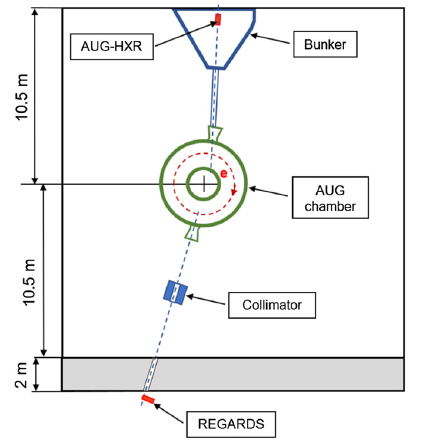
\includegraphics[width=0.52\linewidth]{asdexSpectrometersPosition} }
  \caption{ Расположение гамма-спектрометров на токамаке Asdex Upgrade.~\cite{Shevelev2021} }
  \label{fig:asdexSpectrometersPosition}
\end{figure}

Для уменьшения вклада рассеянных квантов в измеряемый спектр жёсткого рентгена и улучшения реконструкции распределений убегающих электронов был установлен второй спектрометр за биологической защитой токамака ASDEX Upgrade. Спектрометр получил название REGARDS (Runaway Electron GAmma-Ray Detection System)~\cite{DalMolin2019}. Детекторный модуль спектрометра состоит из кристалла LaBr3(Ce) размерами $\varnothing$25$\times$25~мм, соединенного с фотоумножителем Hamamatsu R9420-100-10. Детектор помещен во внешний цилиндрический магнитный экран из мягкого железа. Детектор смотрит на камеру токамака через отверстие в биологической защите диаметром 70~мм. В отверстие вставлен свинцовый коллиматор длиной 10~см диаметром 10~мм. Аппаратная часть системы сбора данных спектрометра REGARDS основана на шасси NI~PXIe-1082, в которое установлен контроллер NI~PXIe-8840 и плата АЦП NI5772-02 с модулем NI PXIe-7966 FlexRIO. Прошивка платы АЦП, разработанная средствами LabView, обеспечивает работу с одним каналом с частотой дискретизации 800~МГц, 400~МГц, 200~МГц, 100~МГц. Работа с двумя каналами возможна на частотах 400~МГц, 200~МГц и 100~МГц. Запись одного отсчёта 12-битной АЦП занимает 2~байта. Для сбора данных с детектора LaBr3(Ce) был выбран режим работы с одним каналом на частоте 400~МГц.~\cite{Shevelev2021}

Усиление детектора контролируется во время разряда плазмы с помощью системы регулировки усиления, состоящей из генератора электрических импульсов, светодиода и оптоволокна. Генератор импульсов используется для запуска светодиода с постоянной частотой 10~кГц. Свет, излучаемый светодиодом, направляется через оптоволокно на фотокатод ФЭУ. Во время анализа сигнала стабильность усиления детектора можно оценить, извлекая импульсы светодиода с помощью методов распознавания формы импульса (форма импульса сигнала от светодиода отличается от формы импульса от регистрации гамма кванта) и контролируя их относительную величину. Эту систему также можно использовать для коррекции небольших сдвигов усиления. Алгоритмы коррекции были реализованы в компьютерном коде DeGaSum.~\cite{Shevelev2021}

% ----------------------------------------------------------

\subsection{Сохранение записываемых осциллограмм}

Поток данных с АЦП составляет $400 \cdot 10^6 \times 2 = 800 \cdot 10^6$~байт в секунду. Записать такой поток данных без предварительной обработки на SSD диск контроллера NI~PXIe-8840 (по сути, персонального компьютера, установленного в крейт) оказалось невозможно --- скорость записи на диск оказалась недостаточной. На борту контроллера имелось 8~Гб оперативной памяти, что недостаточно для сохранения данных с разряда длительностью 10 или 20 секунд данных ($16 \cdot 10^9$~байт). Поэтому требовалось применить дополнительную предобработку записываемых данных, чтобы сохранить осциллограмму за весь разряд токамака без потерь. 

Одним из вариантов такой обработки является сохранение не всей осциллограммы, а только её части. Для этого выбирается некий уровень дискриминации, который больше уровня шумов. Когда значение сигнала превышает уровень дискриминации, сохраняется участок сигнала некой длины. Для удобства обработки нужно сохранять не только сигнал выше уровня, но и участок сигнала перед и после момента превышения уровня (то есть окрестности сигнала, включая как фронт, так и хвост сигнала). Такой способ можно зазвать ``сегментной модой'', он уже был упомянут выше~\cite{Pereira2008}; в упомянутой реализации при сохранении сигнала единичный сегмент данных состоит из 64-битной временной метки, за которой следует 128 16-битных отсчётов АЦП, однако в принципе конкретная реализация сегментной моды может быть и иной (иной размер меток и длины сегмента). Принципиальный недостаток этого способа заключается в том, что при высокой загрузке детектора значение сигнала почти всегда превышает уровень дискриминации, так что фактически сегментная мода вырождается в непрерывную запись и не даёт никаких преимуществ.
 
Поэтому нами был использован другой способ. Для уменьшения объёма сохраняемых данных использовалось сжатие сигнала. Заметим что значение сигнала $s_i$ может быть любым, однако сигнал меняется сравнительно плавно, то есть значение $s'_i = s_i - s_{i-1}$ (первая производной сигнала по времени) обычно сравнительно мало. И если для сохранения значения $s_i$ требуется 2 байта, то для сохранения значения $s'_i$ как правило будет достаточно одного байта. Эта идея лежит в основе дифференциального кодирования~\cite{Sayood2012}. На практике для сигнала сцинтилляционного детектора лучше подходит модификация данного алгоритма --- двойное дифференциальное кодирование, когда сохраняется значение не первой, а второй производной сигнала: $s''_i = (s_i - s_{i-1}) - (s_{i-1} - s_{i-2}) = s_i - 2 s_{i-1} + s_{i-2}$. Остаётся решить вопрос, что делать в ситуации, когда сохраняемое значение второй производной сигнала оказывается вне интервала 
\begin{equation}
  \label{eq:DoubleCompressionOneByte}
  -2^{7}+1 \le s''_i \le +2^7-1 
\end{equation}
и не может быть записано с помощью одного байта. В этой ситуации можно записывать маркерное однобайтовое значение значение (например, $-2^7 = -128$), за которым следуют значения сигнала: $ -2^7, s_i, s_{i+1} $. В этом случае вместо выигрыша в размере записываемых данных (4 байта на 2 отсчёта) наоборот требуется записать больше байт (5 байт на 2 отсчёта из-за наличия маркерного байта); для того, чтобы двойное дифференциальное кодирование приводило к уменьшению размера сохраняемых данных, требуется чтобы ситуации с невыполнением условия~\ref{eq:DoubleCompressionOneByte} случались редко.~\cite{Khilkevich2019Dvp}

Для упрощения сохранения данных и для повышения устойчивости к различным сбоям, данные можно разбить на независимые блоки фиксированного размера $N$~байт. В начале каждого блока находится заголовок с информацией о способе кодирования и временной меткой, за которым следуют данные $s''_i$. При двойном дифференциальном кодировании в начале блока записывается первые два отсчёта $s_1, s_2$ в исходном виде, за которыми следуют закодированные данные. Для декодирования следует вычислить выражение $s_i = s''_i + 2 s_{i-1} - s_{i-2}, i \ge 3$.~\cite{Khilkevich2019Dvp,Shevelev2021}

Размер записываемой осциллограммы можно ещё уменьшить, если данные сжать алгоритмом Deflate~\cite{RFC1951}. 

В результате применения описанных выше методик средний размер записываемых данных за один разряд составляет в среднем примерно 3.8~Гб при записи с одного канала АЦП в течении 10 секунд на частоте 400~МГц ($4\cdot10^9$~отсчётов, $8\cdot10^9$~байт несжатых данных). Удаётся записывать данные без потерь. Имеется возможность увеличить при необходимости время записи до 20 секунд и более.~\cite{Shevelev2021}

Описанные методики сжатия данных были реализованы в компьютерной программе DeGaSum. Управляющая программа детектора REGARDS на основе программы DeGaSum в цикле ожидает прихода стартового триггера на плату АЦП, считывает данные с АЦП в течении заданного времени, и сохраняет осциллограмму в файле, который может быть впоследствии обработан для получения спектров и восстановления функции распределения убегающих электронов по энергии.

% ==========================================================

\section{Восстановление функции распределения убегающих электронов на токамаке ASDEX Upgrade}

После записи осциллограммы обрабатываются, в результате обработки получается массив событий ``время--амплитуда''. Обработка осциллограммы выполняется с помощью программы DeGaSum, алгоритмы обработки подробно описаны в главе~\ref{ch:ch2}. Затем строятся энергетические спектры жёсткого рентгеновского излучения, по которым восстанавливаются функции распределения убегающих электронов. Восстановление производится с помощью программы DeGaSum по алгоритмам, подробно описанным в разделе~\ref{ch:ch3}.

Для реконструкции распределения энергии убегающих электронов в плазме токамака ASDEX Upgrade для обоих детекторов были проведены расчеты методом Монте-Карло функций отклика детектора, генерации тормозного излучения в камере токамака и переноса излучения к детектору. Расчеты проводились А.~Шевелевым с помощью кода MCNP6, для расчёта были разработаны соответствующие модели. Для детектора, установленного в бункере за рентгеновским спектрометром Брэгга, модель MCNP включала подробное описание детектора с кристаллом LaBr3(Ce) $\varnothing$25$\times$17~мм, фотоумножителем и магнитным экраном, установленным на деревянной полке, закрепленной на стене позади спектрометра Брэгга. Для проверки соответствия модели были восстановлены спектры калибровочного источника гамма-излучения ${}^{60}$Co. Для этого в модели детектора был описан точечный источник гамма-излучения, расположенный на расстоянии 5.5~см от боковой поверхности кристалла. Расчеты функций отклика детектора проводились в диапазоне 0.1--2.0~МэВ с шагом по энергии, равным 20~кэВ. На рисунке~\ref{fig:asdex60CoRecostructionBragg} представлены спектр, зарегистрированный спектрометром (после вычитания естественного гамма-фона), и восстановленный исходный спектр источника ${}^{60}$Co (линии 1.173 и 1.332~МэВ). Интегральное значение ошибок восстановления в диапазоне 0.35--1.1~МэВ составляет около 5\%. Эти ошибки можно объяснить неточностью описания местоположения источника в модели. Для расчета переноса жесткого рентгеновского излучения из камеры токамака в детектор была разработана детальная модель коллиматора брэгговского спектрометра.~\cite{Shevelev2021}

\begin{figure}[ht!]
  \centerfloat{ 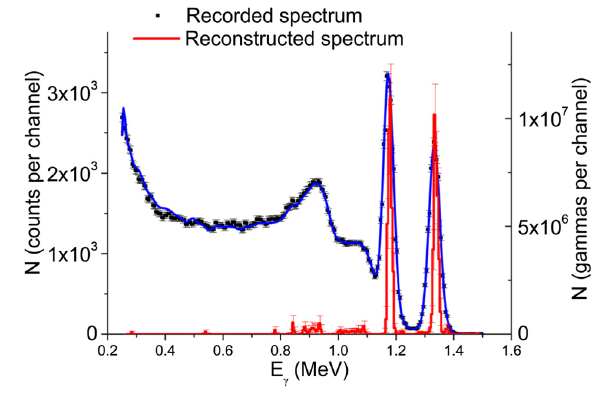
\includegraphics[width=0.72\linewidth]{asdex60CoRecostructionBragg} }
  \caption{ Спектр источника ${}^{60}$Co, зарегистрированный спектрометром LaBr3(Ce) (черные точки, левая ось), и результат восстановления исходного спектра излучения с помощью коду DeGaSum с использованием рассчитанных функций отклика детектора (красная линия, правая ось). Синяя линия --- свертка восстановленного спектра с функциями отклика детектора.~\cite{Shevelev2021} }
  \label{fig:asdex60CoRecostructionBragg}
\end{figure}

Для спектрометра REGARDS модель MCNP включает свинцовый коллиматор длиной 10~см с апертурой $\varnothing$10~мм, размещенный в отверстии в стенке биозащиты токамака. Ось симметрии кристалла детектора вместе с ФЭУ перпендикулярна оси коллиматора. Размеры кристалла LaBr3(Ce) --- $\varnothing$25$\times$25~мм. В экспериментальном зале токамака Asdex Upgrade установлен дополнительный коллиматор из полиэтилена и свинцовых блоков~\cite{Tardini2012}. Для восстановления спектров жёсткого рентгена из плазмы АУГ были рассчитаны функции отклика на моноэнергетическое излучение в диапазоне 0.1--30~МэВ с шагом 0.1~МэВ для обоих детекторов. 

\begin{figure}[ht!]
  \centerfloat{ 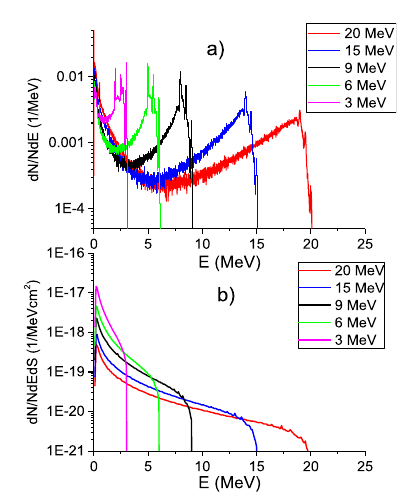
\includegraphics[width=0.52\linewidth]{asdexRegardsResponses} }
  \caption{ Результаты расчетов MCNP: (a) функции отклика детектора LaBr3(Ce) для квантов с энергиями 3, 6, 9, 15 и 20~МэВ; (b) распределения тормозного излучения в месте установки детектора REGARDS, соответствующие взаимодействию моноэнергетических убегающих электронов с энергиями 3, 6, 9, 15 и 20~МэВ с аргоном плазмы.~\cite{Shevelev2021} }
  \label{fig:asdexRegardsResponses}
\end{figure}

Для получения функций в MCNP было смоделировано несколько физических процессов с учетом геометрии вакуумной камеры токамака и расположения детектора. В ходе моделирования было учтено взаимодействие моноэнергетических электронов с газообразной аргоновой мишенью плотностью $10^{20}$~м${}^{-3}$, генерация тормозного излучения и перенос излучения к месту расположения детектора, включая коллиматор и промежуточные материалы. Поскольку сечение генерации тормозного излучения пропорционально $Z^2$ мишени, основной вклад в генерацию излучения вносит инжектируемая примесь аргона, а наличие дейтерия в плазме считалось пренебрежимо малым. В расчетах моделировалось прохождение пучка моноэнергетических электронов через газовую мишень в видимом для детектора объеме камеры токамака. Направление движения электронов в пучке считалось для целей моделирования перпендикулярным направлению обзора детектора, в расчетах не учитывалось питч-угловое распределение относительно тороидальной магнитной оси. Код MCNP использовался для расчета распределения рентгеновского излучения в месте расположения кристаллов обоих детекторов в диапазоне энергий 0.1--30~МэВ с шагом 0.1~МэВ. 

На рисунке~\ref{fig:asdexRegardsResponses} приведены примеры функций отклика спектрометра REGARDS на моноэнергетическое гамма-излучение и распределения тормозного излучения в месте расположения кристалла детектора, рассчитанные для моноэнергетических электронов. На рисунке~\ref{fig:asdexRegardsReSpectrumExamples} показан пример восстановления функции распределения убегающих электронов по энергии.

\begin{figure}[ht!]
  \centerfloat{ 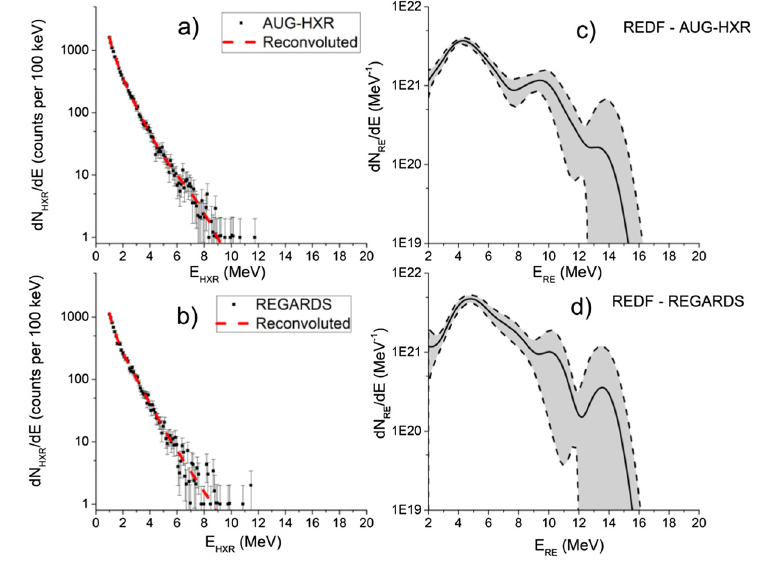
\includegraphics[width=0.72\linewidth]{asdexRegardsReSpectrumExamples} }
  \caption{ Реконструкция функции распределения убегающих электронов по энергии из спектров жёсткого рентгеновского излучения, которые были измерены с помощью спектрометров AUG-UXR и REGARDS. Разряд 36431, временное окно 1.03--1.06~с. (a) спектр жёсткого рентгеновского излучения, измеренный спектрометром AUG-HXR (черные точки); (b) спектр жёсткого рентгеновского излучения, измеренный спектрометром REGARDS (черные точки); (c) функция распределения убегающих электронов, восстановленная кодом DeGaSum из спектра, измеренного детектором AUG-HXR (a); (d) функция распределения убегающих электронов, восстановленная кодом DeGaSum из спектра, измеренного детектором REGARDS (b). Красным пунктиром показан результат свёртки полученной функции распределения с функцией отклика детектора, серой областью на рисунках (c) и (d) показаны границы ошибки восстановленного спектра.~\cite{Shevelev2021} }
  \label{fig:asdexRegardsReSpectrumExamples}
\end{figure}

\FloatBarrier

% ==========================================================

\section{Оценка плотности аргона в плазме}

Убегающие электроны генерировались в токамаке Asdex Upgrade путем инжекции от $3 \cdot 10^{20}$ до $4.8 \cdot 10^{21}$ атомов аргона в плазму низкой плотности. Ток по плазме составлял $I_p = 0.7-0.8$~МА, плотность, усредненная по линии, равна $n_e = 2-4 \cdot 10^{19}$~м${}^{-3}$, тороидальное магнитное поле $B_t = 2.5$~Тл, подводимая мощности электрон-циклотронного нагрева $\approx 2.3$~МВт, $R_0 = 1.61-1.63$~м, $a = 0.55-0.56$~м \cite{Pautasso2020}. Добавление такого тяжелого газа, как аргон, значительно увеличивает потери энергии ускоренными электронами за счет рассеяния и излучения. Для анализа динамики ускорения убегающих электронов необходимо знать плотности компонентов плазмы. Задача усложняется тем, что детекторы наблюдают только относительно небольшой участок плазмы. Детектор AUG-HXR наблюдает примерно 10~см столба плазмы в вертикальном направлении; для спектрометра REGARDS толщина наблюдаемого объёма составляет около 15~см. Кроме того, при низких энергиях $E_{RE} < 1$~МэВ спектрометры не дают надежных данных о количестве убегающих электронов.~\cite{Shevelev2021}

Для оценки доли убегающих электронов, видимых на спектрометре AUG-HXR, были проанализированы сигналы, зарегистрированные в разряде №~34140 (рисунок~\ref{fig:asdexPlasmaParamsPulse34140}). В этом разряде повторно инжектировался аргон в течение 1.07~с. Его усвоение, согласно анализу из работы~\cite{Pautasso2020}, составило~10\%. Благодаря инжектированному аргону средняя плотность плазмы составляла величину $6.6\cdot 10^{20}$~м${}^{-3}$, объём плазмы 3.5~м${}^3$ в момент времени $t = 1.07$~с. Плотность нейтрального аргона (90\% от закачиваемого) составила $5.2\cdot 10^{20}$~м${}^{-3}$, считается что он равномерно распределён по всему объему камеры, который равен 41~м${}^3$. Таким образом, усредненная по видимому столбу плазмы полная плотность аргона составила около $11.7 \cdot 10^{20}$ м${}^{-3}$. Для этой плотности аргоновой мишени и для этого интервала времени по измерениям AUG-HXR был рассчитан ток убегающих электронов. Ток был рассчитан как 
\begin{equation*}
  I_{RE} = e \cdot N_{RE} / \Delta t
\end{equation*}
где $e$ --- заряд электрона, $\Delta t$ --- время набора спектра, $N_{RE}$ --- число электронов, которое было получено после восстановления функции распределения убегающих электронов по измеренному спектру жёсткого рентгеновского излучения:
\begin{equation*}
  N_{RE} = \frac{ n_{Ar} }{ n_{Ar}^{model} } \int \limits_{\varepsilon_{min}}^{\varepsilon_{max}} f_{RE}( \varepsilon ) d\varepsilon
\end{equation*}
где $n_{Ar}$ --- плотность аргона в разряде, $n_{Ar}^{model}$ --- плотность аргона, которая была заложена в код MCNP при вычислении функции отклика, $ \varepsilon_{min} = 0.5$~МэВ и $ \varepsilon_{max} = 30$~МэВ --- пределы, в которых функция распределения убегающих электронов может быть надёжно получена с помощью диагностики по жёсткому рентгеновскому излучению. Для восстановления функции распределения $f_{RE}$ использовался компьютерный код DeGaSum.~\cite{Shevelev2021}
 
\begin{figure}[ht!]
  \centerfloat{ 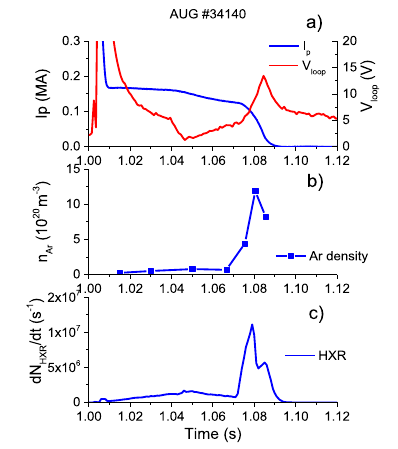
\includegraphics[width=0.72\linewidth]{asdexPlasmaParamsPulse34140} }
  \caption{ Сигналы диагностик в разряде №~34140: a --- ток плазмы (синяя линия) и напряжение обхода (красная линия) после инжекции аргона при $t = 1$~с разряда; (b) --- плотность аргона, восстановленная из измерений жётского рентгена в месте расположения пучка убегающих электронов, видимого для детектора AUG-HXR; (c) временная зависимость скорости счета спектрометра AUG-HXR.~\cite{Shevelev2021} }
  \label{fig:asdexPlasmaParamsPulse34140}
\end{figure}

Повторная инжекция аргона вызвала резкий всплеск жесткого рентгеновского излучения, на порядок превышающий интенсивность излучения до этой повторной инжекции. Максимум излучения пришёлся на 1.079~с разряда, через 9~мс после начала инжекции. В предположении, что убегающие электроны переносят весь ток плазмы, ток убегающих электронов, сигнал от которого регистрируется спектрометром, можно описать как $I_{RE} = k_{det} \cdot I_p$, где $k_{det}$ --- коэффициент, характеризующий долю видимых спектрометром убегающих электронов с учетом порога энергии обнаружения. Для детектора AUG-HXR этот коэффициент был определён равным значению $k_{det} = 0.37$.

Значение 0.37 выглядит завышенным, так как спектрометр AUG-HXR имеет узкий угол обзора и в его поле видимости находится только небольшой объём плазмы. Для коррекции этого значения $k_{det}$ был обработан разряд №~34183 с серией инжекций пеллетов дейтерия. На рисунке~\ref{fig:asdexPlasmaParamsPulse34183} показаны сигналы, зарегистрированные во время этого разряда. После газонапуска аргона, которая вызвала генерацию пучка убегающих электронов с начальным током 0.25~МА, в плазму были инжектированы 15~таблеток замороженного дейтерия с частотой 70~Гц \cite{Pautasso2020}. Пеллеты содержали по $5 \cdot 10^{20}$ молекул дейтерия каждая, в общей сложности --- $1.5 \cdot 10^{22}$ атомов дейтерия, что при равномерном распределении по камере объемом 41~м${}^3$ дает плотность $3.7 \cdot 10^{20}$~м${}^{-3}$. Количество атомов аргона, инжектируемых для генерации пучка убегающих электронов, составляет $7.44 \cdot 10^{20}$. Равномерное распределение аргона по объему камеры дает плотность $1.82 \cdot 10^{19}$~м${}^{-3}$.~\cite{Shevelev2021} 

После обработки спектров жёсткого рентгеновского излучения и зная значение $k_{det}$, можно получить информацию об эволюции плотности аргона. $n_{Ar}$ достигает максимума через 50~мс после начала газонапуска и составляет $0.93 \cdot 10^{20}$~м${}^{-3}$. Если предположить, что это --- средняя концентрация по объему плазмы $\approx 5$~м${}^3$, то она соответствует доли в 62.5\% вдуваемого аргона. Это совпадает с оценкой эффективности напуска аргона после первой инжекции, равной $60 \pm 20$\%, приведенной в~\cite{Pautasso2020}. Затем при инжекции пеллетов дейтерия происходит достаточно быстрое уменьшение плотности аргона, после чего примерно с момента времени $1.15$~с плотность изменяется слабо. Одновременно плотность свободных электронов становится близкой к нулю, что свидетельствует о нейтрализации газовой смеси в токамаке. К моменту времени $1.3$~с разряда плотность аргона достигает минимума $0.6 \cdot 10^{19}$~м${}^{-3}$, что заметно ниже оценки равномерного распределения аргона по камере токамака, которая равна $1.82 \cdot 10^{19}$~м${}^{-3}$, и приведена на рисунке~\ref{fig:asdexPlasmaParamsPulse34183}, (a) зеленой пунктирной линией. Такое несоответствие могло быть вызвано неверным значением $k_{det}$. Для того, чтобы полученная плотность аргона в конце разряда была равна равномерно распределенной концентрации нейтрального аргона, значение $k_{det}$ должно быть равным~0.12.~\cite{Shevelev2021}

\begin{figure}[ht!]
  \centerfloat{ 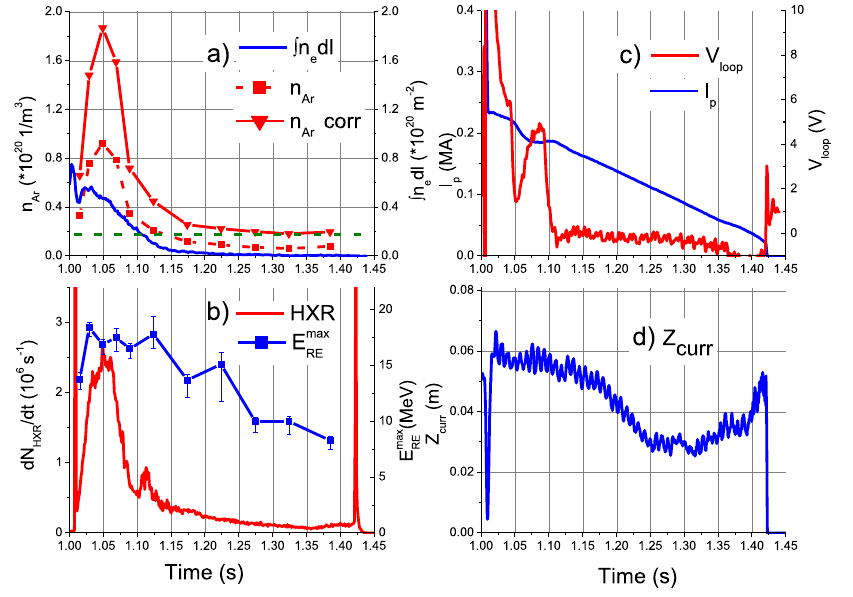
\includegraphics[width=0.82\linewidth]{asdexPlasmaParamsPulse34183} }
  \caption{ Сигналы разряда ASDEX Upgrade №~34183: (a) --- линейная интегральная плотность электронов (синяя линия) и плотность аргона, оцененная по измерениям HXR для $k_det = 0,37$ (красная пунктирная линия с точками) и для скорректированного $k_{det} = 0.12-0.18$ (красная линия с точками). Зеленая пунктирная линия показывает плотность вдуваемого аргона, равномерно распределенную по объему камеры; (b) скорость счета детектора AUG-HXR (красная линия) и полученный максимум $E_{RE}^{max}$ (синяя линия с точками); (c) ток плазмы (синяя линия) и напряжение контура (красная линия); (d) вертикальное положение плазменного потока относительно экваториальной плоскости.~\cite{Shevelev2021} }
  \label{fig:asdexPlasmaParamsPulse34183}
\end{figure}

Для корректировки значения $k_{det}$ и изучения влияния размера и положения пучка убегающих электронов на поток жёсткого рентгена, поступающий на детекторы, было проведено моделирование компьютерным кодом MCNP. Пучок электронов в модели MCNP имел круглое сечение с гауссовым распределением частиц по радиусу. Рассматривались три варианта распределения: при полной ширине на полувысоте (FWHM) потока электронов 10, 15 и 20~см. В модели использовалось реалистичное распределение убегающих электронов, полученное в одном из разрядов токамака Asdex Upgrade с максимальной энергией около 19~МэВ. При моделировании поток излучения, падающий на детекторы, рассчитывался при положении центра распределения луча на луче зрения (смещение 0~см) и смещениях по вертикали 2.5, 5, 7.5, 10, 12,5, 15 и 20~см. Результаты расчетов представлены на рисунке~\ref{fig:asdexModelHxrFlux}. Потоки рентгеновского излучения в месте расположения кристаллов спектрометра нормированы на поток от пучка убегающих электронов с шириной по полувысоте, равной 10~см, взятый без смещения от линии прямой видимости.~\cite{Shevelev2021}

\begin{figure}[ht!]
  \centerfloat{ 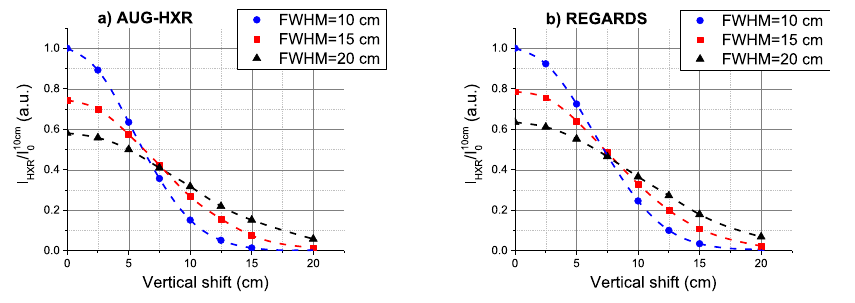
\includegraphics[width=0.95\linewidth]{asdexModelHxrFlux} }
  \caption{ Зависимость потока жёсткого рентгеновского излучения, поступающего на детекторы, от смещения электронного луча с полной шириной на полувысоте, равной 10, 15 и 20~см относительно прямой видимости детекторов AUG-HXR (a) и REGARDS (b).~\cite{Shevelev2021} }
  \label{fig:asdexModelHxrFlux}
\end{figure}

Как видно на рисунке~\ref{fig:asdexModelHxrFlux}, спектрометры более чувствительны к смещениям более узких пучков. В целом в серии разрядов с генерацией убегающих электронов сдвиги пучка относительно экваториальной плоскости не превышали 5--7~см. В работе~\cite{PazSoldan2017} размер и положение пучка электронов в токамаке Asdex Upgrade анализировались по синхротронному излучению, регистрируемому камерой в видимом диапазоне. Диаметр пятна света на полувысоте составлял примерно равен $0.30 a \approx 15$~см при в момент времени $1.029$~с генерацией убегающих электронов. На рисунке~\ref{fig:asdexBeamEvolution34183} показана эволюция равновесия электронного пучка при срыве разряда №34183.~\cite{Shevelev2021}

\begin{figure}[ht!]
  \centerfloat{ 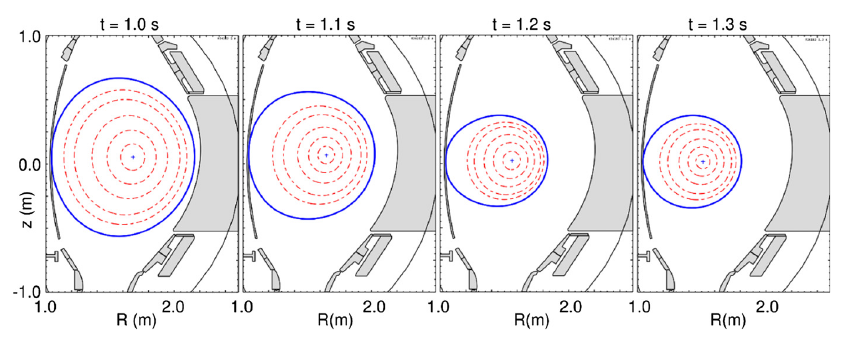
\includegraphics[width=0.95\linewidth]{asdexBeamEvolution34183} }
  \caption{ Эволюция магнитного равновесия пучка убегающих электронов для разряда Asdex Upgrade №34183..~\cite{Shevelev2021} }
  \label{fig:asdexBeamEvolution34183}
\end{figure}

В целом пучёк убегающих электронов продемонстрировал стабильное положение в пространстве. Однако максимальное смещение центра плотности тока относительно положения в начале разрыва составило примерно 3~см в момент 1.3~с разряда (см. рисунок~\ref{fig:asdexPlasmaParamsPulse34183}~(d)). Учитывая начальное смещение пучка относительно оси наблюдения спектрометра на 4~см (линия наблюдения AUG-HXR примерно на 10~см выше экваториальной плоскости токамака), это могло привести к уменьшению числа видимых для детектора электронов в 1.5 раз (соответственно меняется коэффициент $k_{det}$)  при размере пучка на полувысоте $\approx$15~см. Таким образом, камеры в инфракрасном и видимом диапазонах, регистрирующие синхротронное излучение, с помощью которых возможно определить размер и положение пучка убегающих электронов, могут дополнять и корректировать данные рентгеновской диагностики о величине тока убегающих электронов. Используя информацию о положении и размере пучка электронов, было получено скорректированное значение $k_{det}$; после коррекции его значение уменьшилось с 0.18 при $t = 1.05$~с до $0.12$ при $t = 1.3$~с за счет смещения пучка убегающих электронов в пространстве. Полученная в результате эволюция плотности аргона показана на рисунке~\ref{fig:asdexPlasmaParamsPulse34183}~(a) сплошной красной линией с треугольными точками.~\cite{Shevelev2021}

Максимальное значение, достигаемое плотности аргона во время $1,05$~с разряда, составляет $1,87 \cdot 10^{20}$~м${}^{-3}$, что в 2~раза выше полученного ранее $0,93 \cdot 10^{20}$~м${}^{-3}$. Это расхождение объясняется тем, что мы предполагали, что в разряде №34140 ионизированный аргон равномерно распределен по объему плазмы; мы не знали точного значения количества аргона, а только предполагали, что оно составляет около 10\% от количества, введенного во второй раз, и не учитывали влияние смещения пучка убегающих электронов на поток жёсткого рентгеновского излучения, измеряемый детектором. В результате мы получили сильно завышенное значение $k_{det}$. Разумно предположить, что ионизированный аргон находится в области максимальной плотности тока убегающих электронов. При этом среднее значение плотности аргона в объеме плазмы продолжает удовлетворять значению эффективности ионизации $60 \pm 20$\%, приведенному в~\cite{Pautasso2020}. Следует отметить, что объем плазмы, как видно на рисунке~\ref{fig:asdexBeamEvolution34183}, заметно уменьшается при снижении тока убегающих электронов. Так же на значение $k_{det}$ влияет размер пучка убегающих электронов. Для более точного определения размеров и положения пучка убегающих электронов в будущих экспериментах необходимо одновременно измерять жёсткое рентгеновское и синхротронное излучение в инфракрасном/видимом диапазоне.~\cite{Shevelev2021}

\begin{figure}[ht!]
  \centerfloat{ 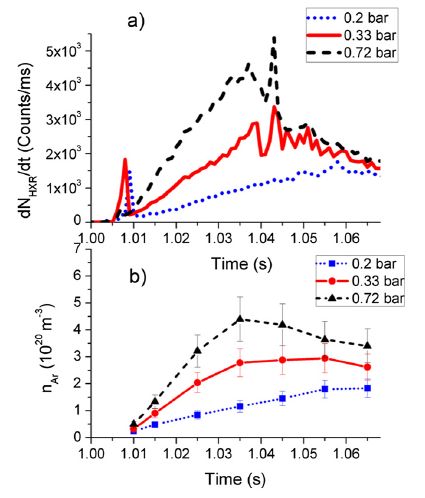
\includegraphics[width=0.52\linewidth]{asdexArgonDensity34183} }
  \caption{ Зависимость скорости счета детектора AUG-HXR от времени (a) и плотности аргона (b) в разрядах с различным количеством инжектируемого аргона на токамаке Asdex Upgrade.~\cite{Shevelev2021} }
  \label{fig:asdexArgonDensity34183}
\end{figure}

На рисунке~\ref{fig:asdexArgonDensity34183}~(b) показано изменение плотности аргона, взаимодействующего с пучком убегающих электронов, восстановленное на основе измерений потока жёсткого рентгеновского излучения, показанного на рисунке~\ref{fig:asdexArgonDensity34183}~(a). Восстановление плотности было проведено начиная с отметки времени  10~мс после подачи аргона. Видно, что с увеличением количества вдуваемого аргона скорость счета детектора жёсткого рентгена пропорционально возрастает и быстрее достигает максимума, что свидетельствует о более быстром увеличении плотности газовой мишени. На $5-9$~мс наблюдаются всплески жёсткого рентгена, которые говорят о выбросах электронов на стенку камеры, сопровождающих МГД-событие. В работе~\cite{Linder2020} описано, что это МГД-событие, по-видимому, вызывает ускоренное проникновение аргона в центральные области плазменного шнура. Наши наблюдения подтверждают это: после вспышек интенсивность жёсткого рентгена быстро возрастает и достигает максимума через $35-55$~мс после инжекции аргона. Через 10~мс после подачи 0,72~бар аргона в разряд №34147 наблюдаемая плотность аргона в центре плазмы составляет $\approx 5 \cdot 10^{19}$ м${}^{-3}$, что согласуется с моделированием проникновения аргона в разряд №33108 с аналогичным количеством закачиваемого газа, которое было проведено в~\cite{Linder2020}.

Таким образом, были проанализированы сигналы жёсткого рентгеновского излучения, измеренные в ходе 19~разрядов с различным количеством инжектированного аргона. Было установлено, что максимальная плотность аргона, взаимодействующего с пучком убегающих электронов, прямо пропорциональна количеству инжектируемого газа (рис. 10). Это свидетельствует о малом вкладе излучения стенки в измеренные спектры жёсткого рентгена.

\begin{figure}[ht!]
  \centerfloat{ 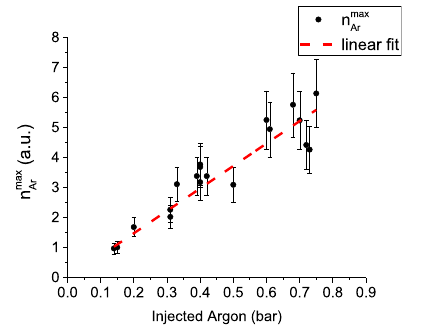
\includegraphics[width=0.52\linewidth]{asdexArgonDensityVsHxr} }
  \caption{ Зависимость максимальной плотности аргона, оцененной с помощью расчетов DeGaSum, от величины подаваемого в токамак аргона.~\cite{Shevelev2021} }
  \label{fig:asdexArgonDensityVsHxr}
\end{figure}


% ==========================================================

\section{Оценка максимальной энергии убегающих электронов}

Проведен анализ ускорения убегающих электронов в разрядах с различными значениями вдуваемого аргона. Эволюция максимальной энергии $E_{max}$ в разряде №~34183, описанном выше, показана на рисунке~\ref{fig:asdexPlasmaParamsPulse34183}~(c) красной линией. Серия инжектированных пеллетов вызвало быструю рекомбинацию аргона, что в, свою очередь, привело к падению плотности электронов и аргона в месте локализации пучка убегающих электронов (рисунок~\ref{fig:asdexPlasmaParamsPulse34183}~(a)).

Уменьшение плотности газа в разряде №~34183 должно уменьшить потери энергии ускоренных электронов на столкновения и тормозное излучение. Однако с момента начала инжекции пеллетов напряжение обхода упало почти до нуля, что предотвратило дальнейшее ускорение электронов. В разряде максимум энергии достигался при 1,02--1,1~с, после чего максимальная энергия электронов постепенно снижалась. 

Были проведены численные расчёты для оценки динамики энергии убегающих электронов с использованием простого 0-D кода PREDICT~\cite{Pandya2019,Patel2021}. В этом коде решаются уравнения движения для тестовой рельятивистской частицы, при этом учитываются потери, вызванные столкновениями и синхротронным излучением. Учитываются различные механизмы генерации убегающих электронов, включающие в себя ускорение в поле Дрейсера, переход в режим убегания электронов из хвоста функции распределения, распад трития, комптоновское рассеяние~(раздел \ref{sec:electronsGeneration}. Использовались следующие уравнения пробных частиц, в которых учитывалось влияние примесей с учетом столкновений убегающих электронов со свободными и связанными электронами и рассеяния на полном и частично экранированном ядерном заряде~\cite{MartinSolis2017,Shevelev2021,Matsuyama2017}:
\begin{equation*}
  \begin{alignedat}{1}
    \frac{ d p_{\parallel} }{ d t } & = e E_{\parallel} - \frac{ e^4 m_e \alpha_e(\gamma) }{ 4 \pi \epsilon_0^2 } \gamma ( Z_{coll}(\gamma) + 1 + \gamma ) \frac{ p_{\parallel} }{ p^3 } - ( F_s + F_b ) \gamma \beta^3 \frac{ p_{\parallel} }{p} \\
    \frac{ d p }{ d t } & = e E_{\parallel} \frac{ p_{\parallel} }{ p } - \frac{ e^4 m_e \alpha_e(\gamma) \gamma^2 }{ 4 \pi \epsilon_0^2 p^2 } - ( F_s + F_b ) \gamma^4 \beta^3 
  \end{alignedat}  
\end{equation*}
где $ p_{\parallel} $ --- компонента импульса, параллельная магнитному (тороидальному) полю, $p$ --- полный импульс убегающего электрона, $\gamma = 1 + p^2 / ( m_e c )^2$ --- релятивистский гамма-фактор, $\beta = v_{RE}/c$, 
\begin{equation*}
  F_s = F_b \left( \frac{ m_e c }{ e B_T R_0 } \right)^2
\end{equation*}
\begin{equation*}
  F_b = \frac{ 2 \varepsilon_0 B_T^2 }{ 3 n_e m_e } \Lambda \frac{ p_{\parallel}^2 }{ p^4 } 
\end{equation*}  
--- вклады синхротронного излучения от движения ведущего центра и от ларморовского движения, $\alpha_e(\gamma)$ и $Z_{coll}(\gamma)$ --- поправочные коэффициенты, учитывающие столкновения убегающих электронов со свободными и связанными электронами, а также рассеяние на полном и частично экранированном ядерном заряде, рассчитанные и описанные в~\cite{MartinSolis2017}. При моделировании вся временная эволюция параметров плазмы использовалась в качестве входных данных, единственным свободным параметром являлась временная эволюция профиля плотности инжектированных атомов аргона.

На рисунке~\ref{fig:asdexForcesEffectsSimulation} показано влияние различных сил, действующих на убегающие электроны. Для электронов, родившихся достаточно рано и успевших ускориться до высоких энергий, увеличение перпендикулярного импульса значительно увеличивает синхротронные потери по сравнению с потерями при столкновениях. Следовательно, присутствие примесей оказывает двоякое влияние на потери энергии убегающими электронами: большее число столкновений снижает их энергию, а питч-угловое рассеяние в присутствии примесей также увеличивает синхротронные потери, особенно для электронов высоких энергий.

\begin{figure}[ht!]
  \centerfloat{ 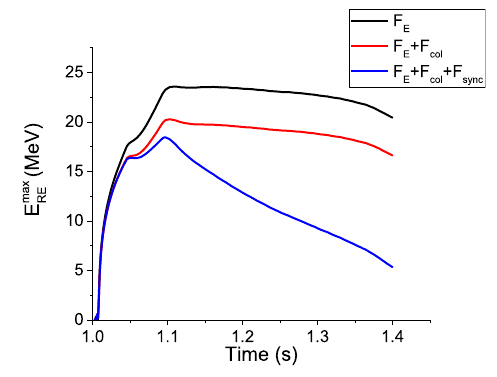
\includegraphics[width=0.52\linewidth]{asdexForcesEffectsSimulation} }
  \caption{ Влияние различных сил на динамику максимальной энергии убегающих электронов. $F_E$ --- сила со стороны электрического поля, $F_{Coll}$ --- сила, возникающая из-за столкновений убегающих электронов с компонентами плазмы, $F_{sync}$ --- сила, возникающая из-за радиационных потерь.~\cite{Shevelev2021} }
  \label{fig:asdexForcesEffectsSimulation}
\end{figure}

Сигналы разряда №~36426 с генерацией убегающих электронов, которая была вызвана инжекцией $9.6 \times 10^{20}$~атомов аргона, показаны на рисунке~\ref{fig:asdexPlasmaParamsPulse36426}. С учетом поправки на смещение пучка убегающих электронов от линии обзора детектора коэффициент $k_{det}$ варьировался в пределах $0,1-0,154$. В то время как спектрометр REGARDS позволяет наблюдать около 15~см столба плазмы против примерно 10~см для спектрометра AUG-HXR, коэффициент $k_{det}$ для REGARDS варьировался в диапазоне $0,15-0,23$. Незначительную разницу в найденной плотности аргона для детекторов, помимо возможных неучтенных ошибок, можно объяснить разным объемом видимой плазмы. Схожие временные зависимости скорости счета обоих детектораов, показанные на рисунке~\ref{fig:asdexPlasmaParamsPulse36426}~(e), свидетельствуют об устойчивом вертикальном положении пучка убегающих электронов.

\begin{figure}[ht!]
  \centerfloat{ 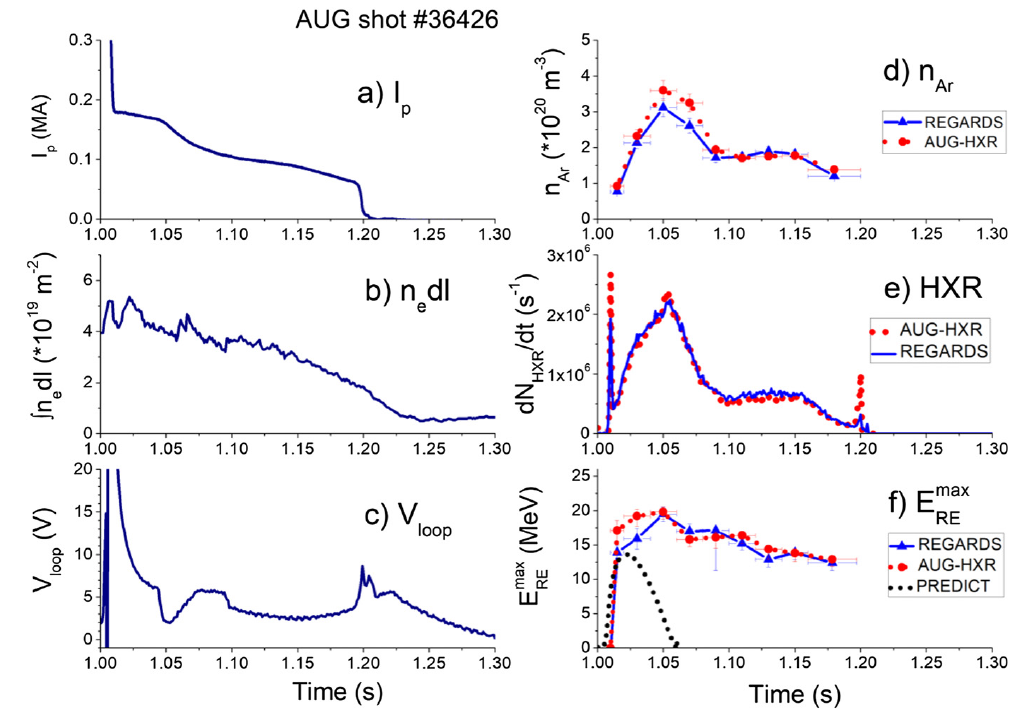
\includegraphics[width=0.92\linewidth]{asdexPlasmaParamsPulse36426} }
  \caption{ Сигналы разряда №~36426: (a) --- ток плазмы; (b) --- линейно интегрированная плотность электронов; (c) --- напряжение обхода; (d) --- плотность аргона в месте локализации пучка убегающих электронов, измеренная по показаниям спектрометров AUG-HXR (красные точки с линией) и REGARDS (синие точки с линией); (e) --- скорость счета спектрометров AUG-HXR (красная линия) и REGARDS (синяя линия); (f) максимальная энергия убегающих электронов, полученная после обработки сигналов спектрометров (точки с линиями) и результаты моделирования метода тестовых частиц с использованием $n_{Ar}$, представленные на рисунке~\ref{fig:asdexArgonDensity34183} (сигнал PREDICT, черная линия).~\cite{Shevelev2021} }
  \label{fig:asdexPlasmaParamsPulse36426}
\end{figure}

Анализ функции распределения убегающих электронов, полученный в результате обработки измеренных спектров с использованием кода DeGaSum, дал временную зависимость максимальной энергии убегающих электронов, показанную на рисунке~\ref{fig:asdexPlasmaParamsPulse36426}~(f). Максимальная энергия убегающих электронов достигает значения в 20~МэВ через 40--60~мс после инжекции аргона, после чего энергия электронов постепенно снижается до $\approx{12,4}$~МэВ в результате потерь на столкновениях с компонентами фоновой плазмы. Однако расчеты, проведенные с использованием кода PREDICT для этой плотности аргона, дали значительно более низкие значения максимальной энергии (рисунок~\ref{fig:asdexPlasmaParamsPulse36426}~(f), черная линия). Согласно этим расчетам, при заданной плотности аргона пучок убегающих электронов должен исчезнуть к $1,07$~с разряда. Расчеты по коду PREDICT показали, что для того, чтобы эволюция максимальной энергии соответствовала измеренным значениям, плотность аргона должна быть на порядок ниже значений, полученных из измерений жёсткого рентгена. Возможная причина подобного расхождения между расчётной и экспериментально наблюдаемой максимальной энергией связана с несколькими факторами, а именно с возможной недооценкой концентрации убегающих электронов в диапазоне низких энергий менее 0,5~МэВ, вкладом питч-угла, который может усиливать эмиссию тормозного излучения в радиальном направлении, взаимодействием убегающих электронов со стенками токамака, вкладом рассеянных квантов в регистрируемый спектр, а так же ошибками в модели пробных частиц. Эти возможные причины находятся в стадии дальнейшего изучения. Тем не менее, результаты настоящего моделирования дают качественное представление о динамике максимальной энергии убегающих электронов при инжекции примеси.

Проанализирована зависимость максимальной энергии убегающих электронов от количества инжектированного аргона в диапазоне от 0,14 до 0,75~бар. Максимальная энергия измеряли в 18~разрядах в интервале времени от 80 до 120~мс после инжекции аргона. Полученная зависимость показана на рисунке~\ref{fig:asdexMaxElectronEnergy}. В целом нельзя сказать, что количество вводимого аргона в этом диапазоне плотностей существенно влияет на максимальную энергию: её значение уменьшается примерно с 18 до 16~МэВ. Также можно отметить сходство в динамике эволюции максимальной энегрии для разрядов с разным количеством вдуваемого аргона (рисунок~\ref{fig:asdexMaxElectronEnergy}~(b)). Эти наблюдения требуют теоретической интерпретации и дополнительных исследований.

\begin{figure}[ht!]
  \centerfloat{ 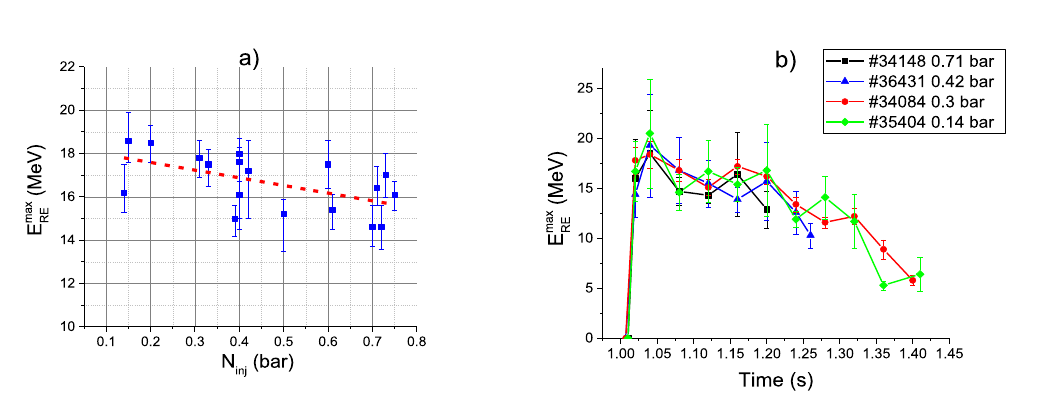
\includegraphics[width=0.92\linewidth]{asdexMaxElectronEnergy} }
  \caption{ Максимальня энергия убегающих электронов $ E_{RE}^{Max}$: (a) --- зависимость максмальной энергии убегающих электронов от количества инжектируемого аргона (красная пунктирная линия --- линейная аппроксимация); (b) --- эволюция максимальной энергии в разрядах с различной инжекцией аргона.~\cite{Shevelev2021} }
  \label{fig:asdexMaxElectronEnergy}
\end{figure}

Следует отметить, что в недавних измерениях синхротронного излучения, проведенных на токамаке Asdex Upgrade~\cite{PazSoldan2017} с помощью светосильной камеры видимого диапазона Phantom V711 (c фильтром узкого диапазона на 708,9~нм с полушириной 8,6~нм), присутствие затравочных начальных электронов с энергиями выше 25~МэВ, тогда как согласно данными со спектрометров жёсткого рентгена за тот же интервал времени  максимальная энергия составляет 16~МэВ. Камера была сконфигурирована в направлении приближения убегающих электронов (тангенциальная линия обзора) и использовалась для наблюдения за синхротронным излучением, и она должна была начать принимать достаточный сигнал синхротронного излучения, как только убегающие электроноы наберут энергию более 25~МэВ с углом наклона 0,2~радиана. Причины такого несоответствия, вероятно, можно объяснить малым числом затравочных электронов высокой энергии в плазме и низкой чувствительностью используемых спектрометров жёсткого рентгеновского излучения к излучению, излучаемому перпендикулярно пучку убегающих электронов.

% ----------------------------------------------------------

\section{Выводы к главе 4}

На токамаке ASDEX Upgrade разработаны и введены в эксплуатацию два спектрометра жёсткого рентгеновского излучения на основе сцинтилляционных кристаллов LaBr3(Ce) небольшого размера. Спектрометры использовались в экспериментах по генерации убегающих электронов в разрядах с малой плотностью плазмы при инжекции небольшого количества аргона. В течение всего разряда сигнал регистрировался с частотой дискретизации 400~МГц. Для амплитудного анализа регистрируемого сигнала в условиях высокой нагрузки спектрометра с большим количеством наложенных импульсов был использован метод фиттинга, позволяющий достичь скорости счета спектрометра $10^7$~с${}^{-1}$ при относительно небольшом числе неразрешённых импульсов. Анализ функции распределения убегающих электронов по энергиям, полученной в результате обработки измеренных спектров с помощью программы DeGaSum, позволил получить зависимость максимальной энергии убегающих электронов от времени. Убегающие электроны достигают максимальной энергии 20~МэВ через 40--60~мс после инжекции аргона, после чего энергия электронов постепенно снижается до $\approx{12,4}$~МэВ.


Полученные распределения убегающих электронов позволили оценить плотность газовой мишени и видимую для спектрометров долю пучка убегающих электронов. Плотность аргона, соответствующая 62.5\% от всего инжектированного аргона, находится в хорошем соответствии с результатами из работы~\cite{Pautasso2020}, и моделью транспорта примесных ионов в центральную плазму, рассмотренной в~\cite{Linder2020}. Получена энергетическая зависимость максимальной энергии убегающих электронов от количества вдуваемого в плазму аргона, которая оказалась не существенной: максимальная энергия уменьшалась примерно на 10\% при увеличении вдувания аргона с 0,14 до 0,73~бар. Численные расчёты с помощью моделирования тестовых частиц, выполненные с использованием кода PREDICT, показали, что для того, чтобы эволюция максимальной энергии соответствовала измеренным значениям, плотность аргона должна быть на порядок ниже значений, полученных по измерениям с помощью жёсткого рентгеновского излучения. Возможные причины такого расхождения находятся в стадии дальнейшего изучения. Тем не менее, результаты настоящего моделирования дают качественное представление о динамике убегающих электронов при тнжекции примеси.

Проведенное измерение продемонстрировало возможность использования малогабаритных спектрометров для диагностики убегающих электронов на более крупных установках, таких как ITER, где разрабатывается система мониторинга жёсткого рентгеновского излучения с кристаллами с аналогичными характеристиками. В настоящей работе весь ток плазмы после инжекции аргона переносился убегающими электронами, что позволило оценить плотность аргона в центре плазмы. В будущих экспериментах на ITER можно будет решить обратную задачу нахождения тока убегающих электронов по измеренному сигналу со спектрометров жёсткого рентгеновского излучения при условии, что известны распределения примесей. Для адекватной оценки тока убегающих электронов необходимо использовать спектрометрическую систему, имеющую не менее двух линий обзора плазмы, в поле наблюдения которой находится всё сечение плазменного столба. Измерение синхротронного излучения в инфракрасном и видимом диапазонах может дополнить информацию о размере и положении пучка убегающих электронов, а также о наличии электронов с энергиями выше 10~МэВ.

% ==========================================================

\FloatBarrier
